\setcounter{chapter}{2}
\chapter{Phân tích hệ thống}
EHAT sẽ sử dụng các bảng có sẵn trong database của hệ thống học tập Moodle để lấy thông tin, phân tích và sẽ trả về những kết quả mà ta mong đợi. Chính vì thế nhóm chúng em sẽ nêu ra những use case cũng như những database của Moodle cần thiết phục vụ cho quá trình xây dựng công cụ EHAT.
\section{Nghiên cứu use case của hệ thống Moodle}
\subsection{Những hành động cơ bản của giáo viên và học sinh có sẵn trên Moodle}
Khi chưa thêm công cụ EHAT giáo viên và học sinh có những hành động cơ bản sau: \cite{usecase:1}
\begin{itemize}
	\item Đối với giáo viên
	\begin{center}
		\begin{figure}[htp]
			\begin{center}
				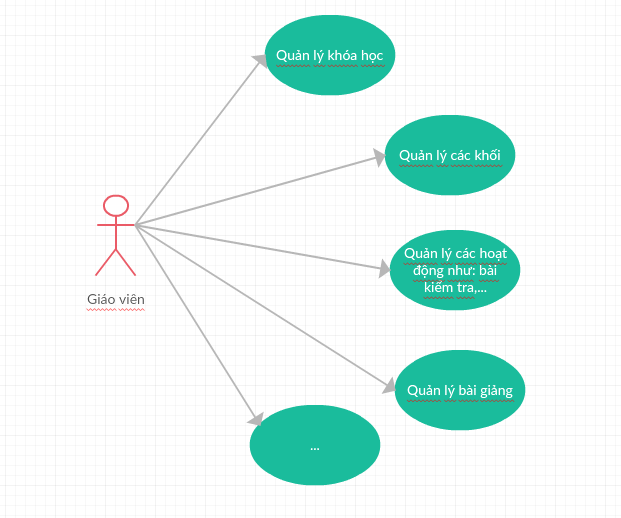
\includegraphics[scale=0.7]{img/usecasegv}
			\end{center}
			\caption{Use case thể hiện hành động cơ bản của GV}
			\label{refhinh10}
		\end{figure}
	\end{center}
	\vskip 1cm 
	\item Đối với học sinh, sinh viên
	\begin{center}
		\begin{figure}[htp]
			\begin{center}
				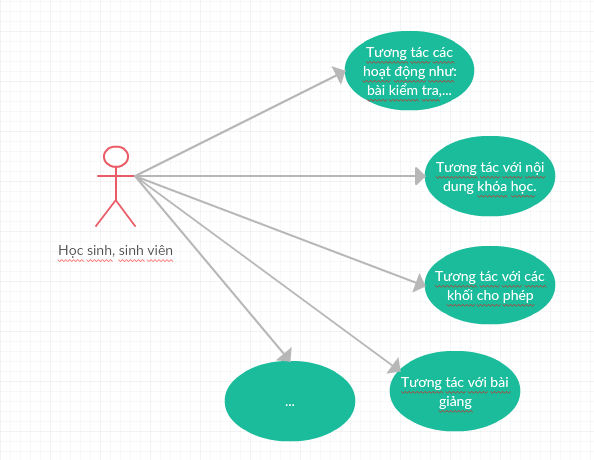
\includegraphics[scale=0.7]{img/usecasehs}
			\end{center}
			\caption{Use case thể hiện hành động cơ bản của HS, SV}
			\label{refhinh11}
		\end{figure}
	\end{center}
\end{itemize}

\subsection{Những hành động khi thêm công cụ EHAT}
Sau khi thêm vào hệ thống công cụ EHAT:
\begin{itemize}
	\item Đối với giáo viên
	\begin{center}
		\begin{figure}[htp]
			\begin{center}
				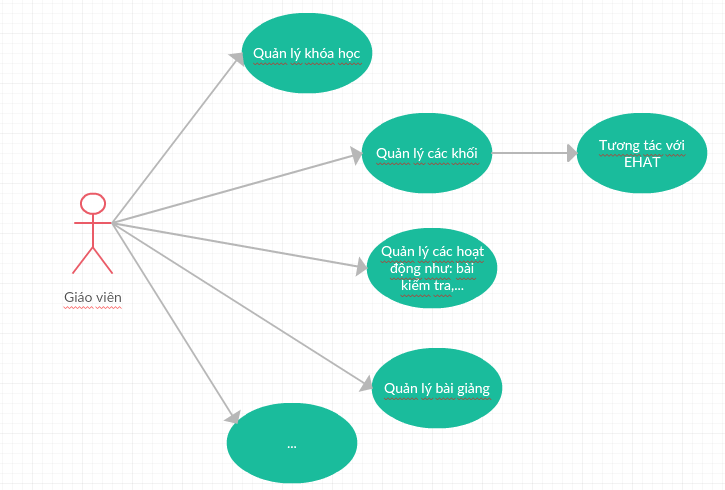
\includegraphics[scale=0.65]{img/usecasegvehat}
			\end{center}
			\caption{Use case thể hiện hành động cơ bản của GV khi có EHAT}
			\label{refhinh12}
		\end{figure}
	\end{center}
	\vskip 3cm
	\item Đối với học sinh, sinh viên
	\begin{center}
		\begin{figure}[htp]
			\begin{center}
				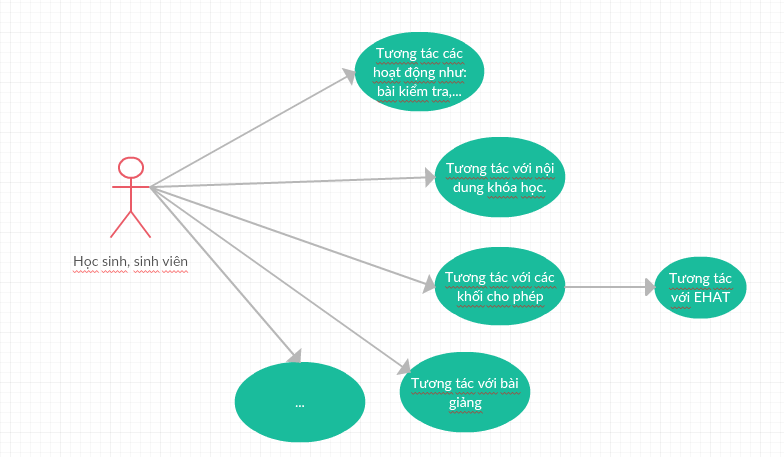
\includegraphics[scale=0.7]{img/usecasehsehat}
			\end{center}
			\caption{Use case thể hiện hành động cơ bản của HS, SV khi có EHAT}
			\label{refhinh13}
		\end{figure}
	\end{center}
\end{itemize}

Chi tiết các hoạt đông mà EHAT mang lại:
\begin{itemize}
	\item Đối với giáo viên
	\begin{center}
		\begin{figure}[htp]
			\begin{center}
				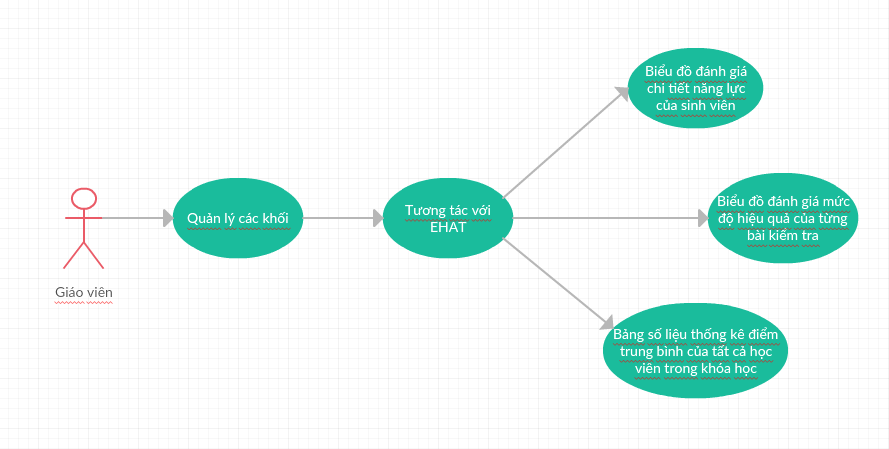
\includegraphics[scale=0.7]{img/chitietehatgv}
			\end{center}
			\caption{Các hoạt động EHAT mang lại cho GV}
			\label{refhinh14}
		\end{figure}
	\end{center}
	\vskip 4cm
	\item Đối với học sinh, sinh viên
	\begin{center}
		\begin{figure}[htp]
			\begin{center}
				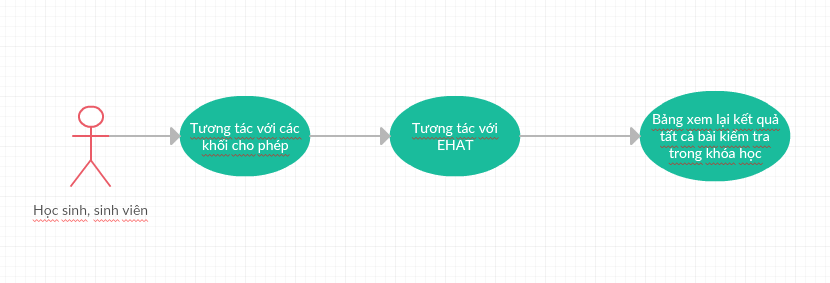
\includegraphics[scale=0.7]{img/chitietehaths}
			\end{center}
			\caption{Các hoạt động EHAT mang lại cho HS, SV}
			\label{refhinh15}
		\end{figure}
	\end{center}
\end{itemize}

\section{Database của Moodle}

\section{Những dạng biểu đồ sẽ được sử dụng trong EHAT}
EHAT sử dụng dữ liệu trong database của Moodle từ những khóa học riêng lẻ để phân tích và xây dựng các biểu đồ để thể hiện các mục tiêu mà ta mong đợi. Để đáp ứng được những mục tiêu đó với từng loại dữ liệu ta sẽ có một dạng biểu đồ tương ứng để có thể phản ảnh rõ nhất đặc điểm của dữ liệu, các dạng biểu đồ mà EHAT sử dụng bao gồm:
\begin{itemize}
	\item Biểu đồ mạng nhện (Radar Chart)
	
	Nhóm chúng em sẽ dùng biểu đồ mạng nhện để áp dụng cho việc đánh giá và so sánh chi tiết năng lực của các HV.
	\begin{center}
		\begin{figure}[htp]
			\begin{center}
				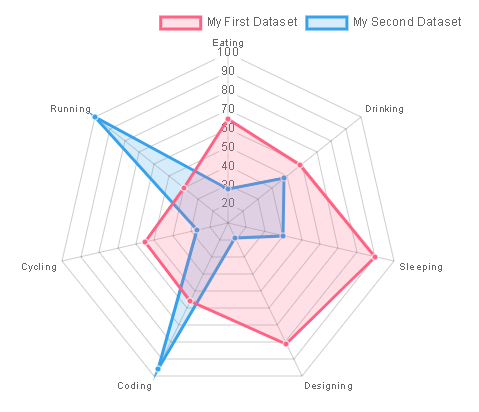
\includegraphics[scale=0.7]{img/radar}
			\end{center}
			\caption{Biểu đồ mạng nhện}
			\label{refhinh16}
		\end{figure}
	\end{center}
	
	\item Biểu đồ cột (Bar Chart)
	
	Biểu đồ cột sẽ được áp dụng cho việc thống kê phần trăm sinh viên có điểm trung bình của từng bài kiểm tra lớn hơn hoặc bằng 5 để dễ dàng đánh giá mức độ hiệu quả của việc xây dựng bài kiểm tra.
	\begin{center}
		\begin{figure}[htp]
			\begin{center}
				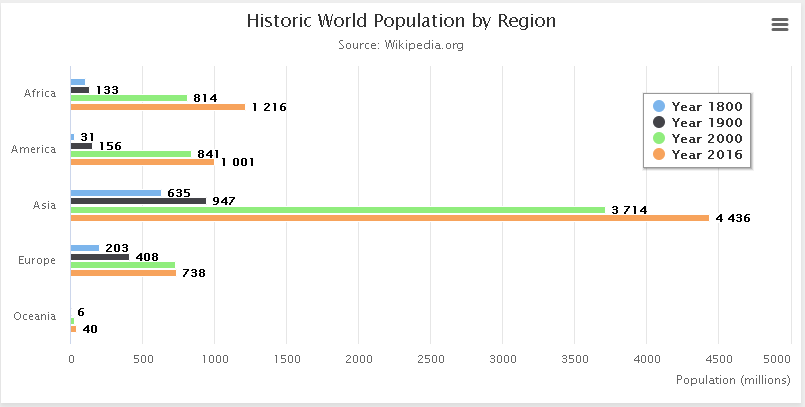
\includegraphics[scale=0.7]{img/bar}
			\end{center}
			\caption{Biểu đồ cột}
			\label{refhinh17}
		\end{figure}
	\end{center}
	
	\item Biểu đồ đường (Line Chart)
	
	Biểu đồ đường được sử dụng cho việc xem xét mức độ học tập hiệu quả của sinh viên đối với khóa học
	\begin{center}
		\begin{figure}[htp]
			\begin{center}
				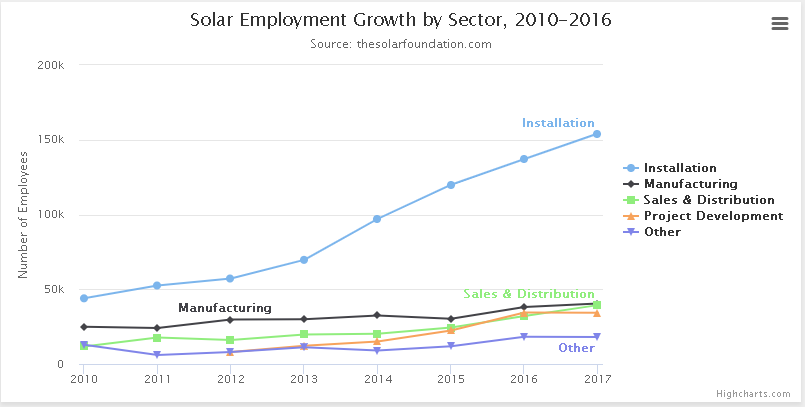
\includegraphics[scale=0.7]{img/line}
			\end{center}
			\caption{Biểu đồ đường}
			\label{refhinh18}
		\end{figure}
	\end{center}
	
\end{itemize}